% Compile with XeLaTeX: latexmk -xelatex WC2026_technical_companion.tex
% Reads side-by-side with WC2026_paper.tex.
\documentclass[11pt,letterpaper]{article}
\usepackage{fontspec}
\setmainfont{Times New Roman}
\usepackage{amsmath}
\usepackage{amssymb}
\usepackage{booktabs}
\usepackage{longtable}
\usepackage[letterpaper,margin=1in]{geometry}
\usepackage{caption}
\usepackage{multirow}
\usepackage{natbib}
\usepackage{graphicx}
\usepackage{float}
\usepackage{pdflscape}
\usepackage{avtables}
\usepackage[hidelinks]{hyperref}
\captionsetup{font=small,labelfont=bf}

% Prefix companion tables/figures with C to avoid collision with main paper
\renewcommand{\thetable}{C\arabic{table}}
\renewcommand{\thefigure}{C\arabic{figure}}

% Code anchor: \anchor{scripts/file.py:function — constants}
\newcommand{\anchor}[1]{%
  \smallskip\noindent\textsc{Anchor.}~\texttt{#1}\smallskip}

% Honesty note block
\newenvironment{honesty}{%
  \begin{quote}\textit{Honesty note.}~}{%
  \end{quote}}

\title{\textbf{Technical Companion:}\\[4pt]
  \large Forecasting the 2026 FIFA World Cup:
  A Market-Calibrated Poisson--Elo Model and
  the Information Each Result Reveals}
\author{Avralt-Od Purevjav \and Jeronimo Luza}
\date{June 2026}

\begin{document}
\maketitle

\begin{abstract}
This document is the mathematical companion to the above paper.
Every pipeline step is presented as the mathematics it implements,
every modeling assumption is stated with its known limitations,
and every formula is anchored to the exact code that executes it.
It reads side-by-side with the paper; section numbers mirror the
paper's stages~0--6 (Part~I) and~7--12 (Part~II).
\end{abstract}

\begin{figure}[H]
\centering
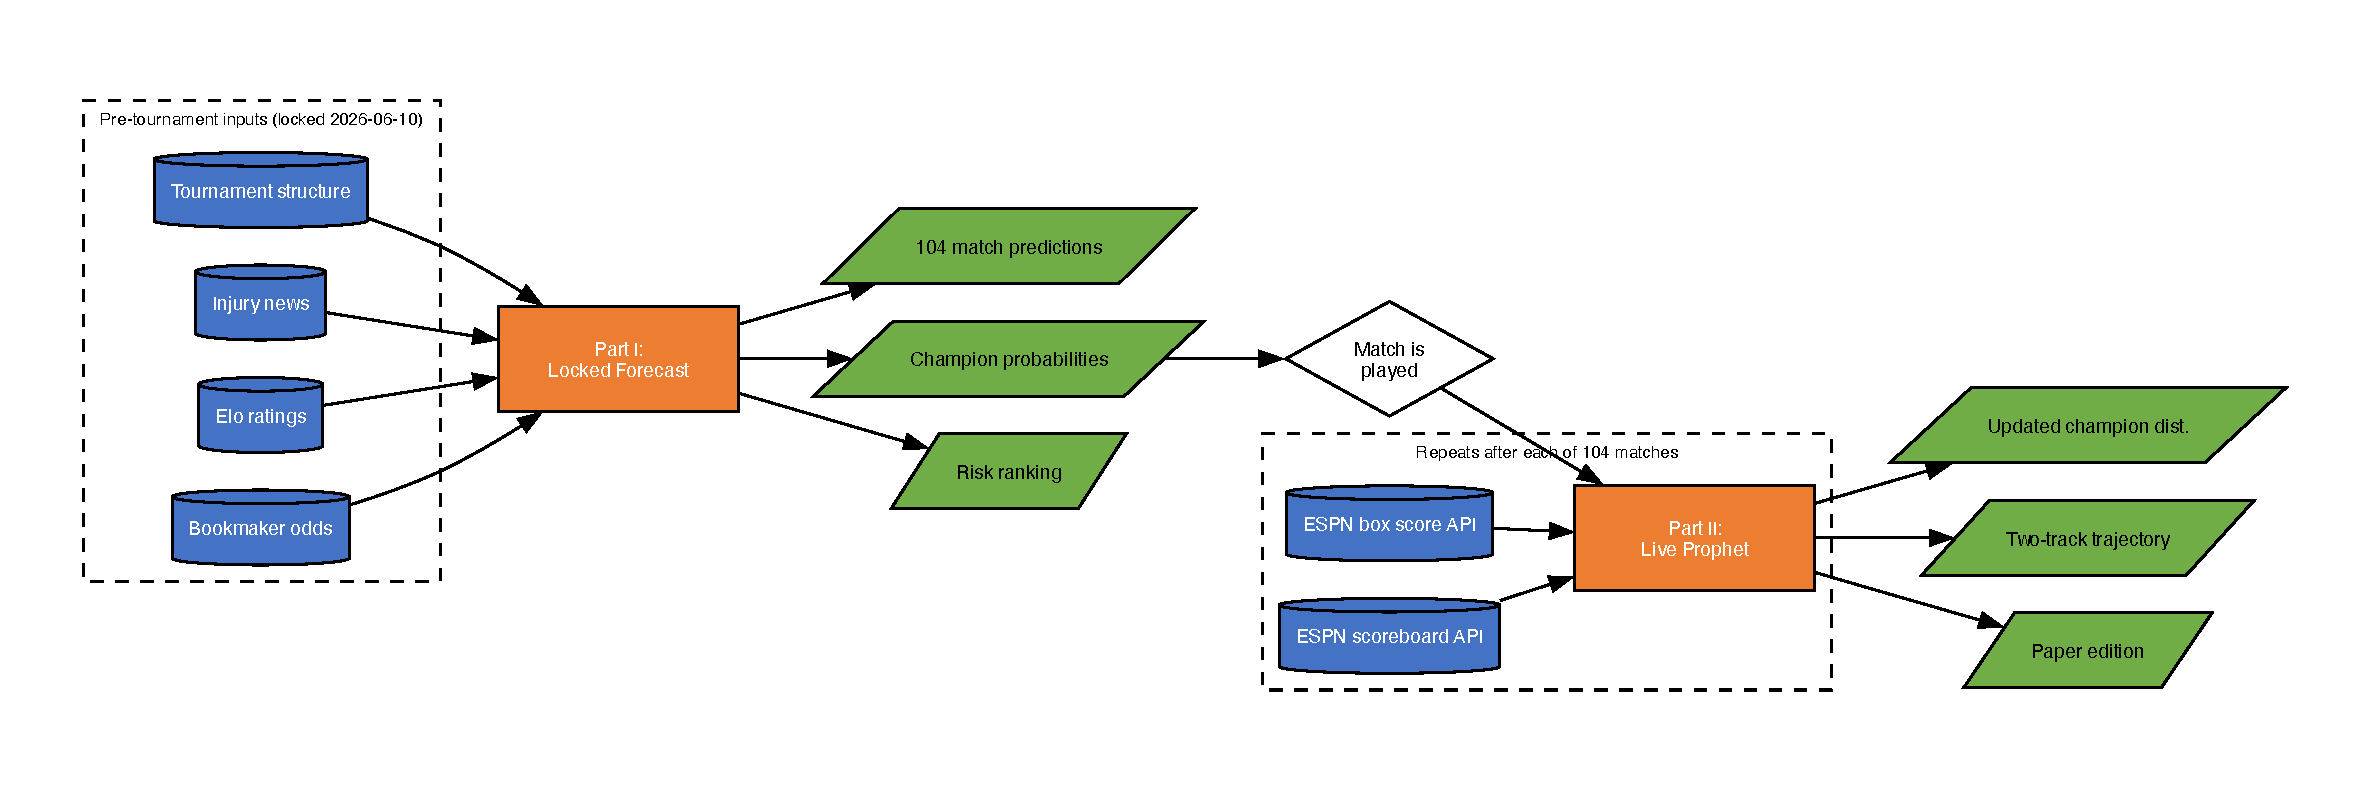
\includegraphics[width=\textwidth]{figs/fig_pipeline_overview.pdf}
\caption{Master overview of the two-phase pipeline. Part~I (locked forecast,
Figure~\ref{fig:part1}) runs once before the tournament; Part~II (live
Prophet, Figure~\ref{fig:part2}) repeats after each of 104 matches.}
\label{fig:overview}
\end{figure}

\tableofcontents
\clearpage

% ── §0 ──────────────────────────────────────────────────────────────────────
\section*{\S 0\quad Notation and contract}
\addcontentsline{toc}{section}{\S 0\enspace Notation and contract}
\label{sec:notation}

Throughout, $i$ indexes teams and $R_i$ is team $i$'s Elo rating (a scalar
strength, e.g.\ Spain~2165, Qatar~1423). A match between designated home
side $H$ and away side $A$ produces a scoreline
$(h,a)\in\mathbb{Z}_{\ge0}^2$. The model's prediction is $(\hat h,\hat a)$.
Goal rates $\lambda_H,\lambda_A>0$ are the expected goals of each side under a
Poisson model. Outcome probabilities are the triple
$(p_H,p_D,p_A)$~--- home win, draw, away win~--- and $o_j$ denotes a decimal
bookmaker odds quote for outcome $j\in\{H,D,A\}$. The pool score function is
$S(\hat h,\hat a;\,h,a)\in\{0,1,2,3\}$ (defined in \S\ref{sec:notation}).
In Part~II, $p_t$ denotes the champion probability distribution over all 48
teams after conditioning on the first $t$ played games, and $d_i$ is team
$i$'s learned rating drift.

Two contracts hold throughout this document:
\begin{enumerate}
\item \textbf{Anchor contract.} Every displayed equation is followed by an
anchor naming the code that implements it --- \texttt{scripts/file.py:function}
--- with the constants as locked before kickoff (2026-06-10). The formulas
are extracted from the code, not from an idealized model.
\item \textbf{Honesty rule.} Where the code is a pragmatic shortcut rather
than clean statistics (an independence assumption, a proportional vig split,
a memoized grid), the note says so explicitly rather than dressing it up.
\end{enumerate}

% ── §0.5 ────────────────────────────────────────────────────────────────────
\section*{\S 0.5\quad Complete variable inventory}
\addcontentsline{toc}{section}{\S 0.5\enspace Complete variable inventory}
\label{sec:inventory}

\subsection*{Tier 1 --- Pre-tournament inputs (locked 2026-06-10)}

\begin{table}[H]
\centering
\caption{Pre-tournament inputs. All files are committed before kickoff
(tag \texttt{prereg-2026}) and never re-read from the outside world.}
\label{tab:tier1}
\small
\begin{tabular}{p{2.8cm}p{3.5cm}p{3.5cm}p{2.5cm}p{2cm}}
\toprule
Symbol & What & How measured & Values / range & File \\
\midrule
$o_H, o_D, o_A$ &
  Bookmaker decimal odds &
  Hand-collected Jun 2--7 from bet365, FanDuel, DraftKings, Betfair,
  Kalshi/Polymarket; one source per fixture, recorded in \texttt{source} field &
  e.g.\ Mexico--S.Africa: 1.40 / 4.60 / 8.00 &
  \texttt{data/odds\_AD.json}, \texttt{odds\_EH.json}, \texttt{odds\_IL.json} \\[4pt]
$R_i$ &
  Elo rating, 48 teams &
  Read from ClubElo/EloRatings.net, Jun 5--7 &
  Spain 2165 \ldots\ Qatar 1423 &
  \texttt{data/elo\_outright\_news.json} \\[4pt]
$\delta_i^{\mathrm{inj}}$ &
  Injury Elo deduction &
  Hand-set scalar per confirmed absence &
  NED $-23$, BRA $-20$, JPN $-10$, CRO $-10$, ESP $-5$ &
  \texttt{data/elo\_outright\_news.json} \\[4pt]
$\delta_i^{\mathrm{mkt}}$ &
  Market recalibration &
  Prediction-market implied 140-pt Portugal--Colombia gap vs.\ Elo
  7-pt $\to$ split &
  POR $+66$, COL $-67$ &
  \texttt{scripts/condition.py} \\[4pt]
$\delta_{\mathrm{host}}$ &
  Host venue bonus &
  Fixed rule; decays in late rounds &
  $+40$ R32/R16; $+20$ QF onward &
  \texttt{scripts/condition.py} \\[4pt]
\textsc{group\_fixtures} &
  72 group fixtures &
  Static table (row, group, home, away) &
  --- &
  \texttt{scripts/fixtures.py} \\[4pt]
\textsc{knockout} &
  32-slot bracket wiring &
  Directed graph, FIFA R32/R16/QF/SF/Final &
  --- &
  \texttt{scripts/fixtures.py} \\
\bottomrule
\end{tabular}
\end{table}

\subsection*{Tier 2 --- Intermediate computed values}

\begin{table}[H]
\centering
\caption{Intermediate values derived during pipeline execution.}
\label{tab:tier2}
\small
\begin{tabular}{p{2.6cm}p{3.2cm}p{5cm}p{2.4cm}}
\toprule
Symbol & What & Formula / source & Range \\
\midrule
$p_H, p_D, p_A$ &
  Fair outcome probabilities &
  $p_j = (1/o_j)/\sum_k(1/o_k)$; or Elo synthesis for odds-free matches &
  $[0,1]$, sum $=1$ \\[4pt]
$\lambda_H, \lambda_A$ &
  Expected goal rates &
  \texttt{fit\_rates}: grid search minimise $\sum(\tilde p_j-p_j)^2$,
  step 0.05, total goals $\in[1.6,3.4]$ &
  0.10--3.50 each \\[4pt]
$P(h,a)$ &
  Scoreline distribution &
  $\mathrm{Pois}(h;\lambda_H)\cdot\mathrm{Pois}(a;\lambda_A)$,
  $(h,a)\in\{0,\ldots,8\}^2$ &
  81 values, sums to $\approx1$ \\[4pt]
$\hat h, \hat a$ &
  Match prediction &
  $\arg\max\,\mathbb{E}[S]$ over $9\times9$ grid (EV rule);
  or modal-conditional; or realistic readout &
  integers 0--8 \\[4pt]
$\mathbb{E}[S(\hat h,\hat a)]$ &
  Expected pool points &
  $p_{\mathrm{exact}}+p_{\mathrm{result+GD}}+p_{\mathrm{result}}$
  (exact, no simulation) &
  $[0,3]$ \\[4pt]
$\lambda_{\mathrm{obs}}$ &
  Observed performance (proxy xG) &
  $0.3256\times\mathrm{SoT}$; calibrated OLS on 236 WC team-matches &
  $\ge0$ \\[4pt]
$\lambda_{\mathrm{exp}}$ &
  Expected performance &
  Elo synthesis $+$ \texttt{fit\_rates} at current $R_i^{\mathrm{eff}}$;
  memoised on integer Elo diff &
  0.10--3.50 \\[4pt]
$s$ &
  Net surprise (home) &
  $(\lambda_{\mathrm{obs}}^H - \lambda_{\mathrm{exp}}^H)
   -(\lambda_{\mathrm{obs}}^A - \lambda_{\mathrm{exp}}^A)$;
  zero-sum by construction &
  $\mathbb{R}$ \\[4pt]
$d_i$ &
  Per-team rating drift &
  $d \leftarrow 0.95\,d + \mathrm{clip}(50\,s,\pm75)$;
  initialised 0 at kickoff &
  $\approx\pm214$ max over group stage \\[4pt]
$R_i^{\mathrm{eff}}$ &
  Effective rating &
  $R_i+\delta_i^{\mathrm{inj}}+\delta_i^{\mathrm{host}}
   +\delta_i^{\mathrm{mkt}}+d_i$ &
  --- \\[4pt]
$p_t$ &
  Champion distribution at time $t$ &
  Monte Carlo counter over $N$ simulations &
  $[0,1]$ over 48 teams, sum $=1$ \\[4pt]
$D_{\mathrm{KL}}(p_t\|p_{t-1})$ &
  Per-game information (bits) &
  $\sum_i p_t(i)\log_2[p_t(i)/\max(p_{t-1}(i),\varepsilon)]$,
  $\varepsilon=10^{-12}$ &
  $\ge0$ bits \\
\bottomrule
\end{tabular}
\end{table}

\subsection*{Tier 3 --- Hyperparameters and tuning constants (locked pre-tournament)}

\begin{table}[H]
\centering
\caption{All constants locked at kickoff (2026-06-10).}
\label{tab:tier3}
\small
\begin{tabular}{llp{7cm}}
\toprule
Constant & Value & Rationale \\
\midrule
\texttt{MAX\_G}       & 8      & Poisson tail $<2.4\times10^{-4}$ at $\lambda=2$ \\
$N_{\mathrm{pre}}$    & 200{,}000 & MC SE $\approx\pm0.1$ pp at champion scale \\
$N_{\mathrm{cond}}$   & 50{,}000  & Per-track post-match re-simulation \\
$N_{\mathrm{replay}}$ & 4{,}000   & Per-snapshot in 2022 replay validation \\
seed                  & 2026   & Fixed for reproducibility \\
$\lambda$ grid step   & 0.05   & Balances inversion precision vs.\ compute \\
total goals band      & $[1.6,3.4]$ & WC group games average $\approx2.5$--2.7 total goals \\
$k$ (learning gain)   & 50     & Midpoint of 2022 optimum (40) and 2018 optimum (60) \\
$\gamma$ (decay)      & 0.95   & Drift half-life $\approx13.5$ matches \\
$B$ (drift bound)     & 75     & Hard clip on per-match step \\
$\varepsilon$ (KL floor) & $10^{-12}$ & Prevents $\log0$ in divergence \\
host bonus early      & $+40$  & R32 and R16 rounds \\
host bonus late       & $+20$  & QF, SF, Final \\
draw share base       & 0.30   & Decays as $e^{-|d|/700}$ with Elo gap \\
pen threshold         & 0.25   & Winner's rate edge $<0.25$ goals $\Rightarrow$ penalties pick \\
\bottomrule
\end{tabular}
\end{table}

% ── §0.6 ────────────────────────────────────────────────────────────────────
\section*{\S 0.6\quad Match lifecycle variables}
\addcontentsline{toc}{section}{\S 0.6\enspace Match lifecycle variables}
\label{sec:lifecycle}

\subsection*{\S 0.6a --- Before-game state (entering match $m$)}

\begin{table}[H]
\centering
\caption{Variables the model knows entering match $m$, and whether they update
after each prior match.}
\label{tab:before}
\small
\begin{tabular}{p{2.8cm}p{3.2cm}p{4.5cm}p{2cm}}
\toprule
Symbol & What & How determined & Updated\\
 & & & each match? \\
\midrule
$R_i$ &
  Baseline Elo &
  Locked Jun 10, from \texttt{elo\_outright\_news.json} &
  No \\[4pt]
$\delta_i^{\mathrm{inj}}$ &
  Injury deduction &
  Hand-set pre-tournament &
  No \\[4pt]
$\delta_i^{\mathrm{host}}$ &
  Host venue bonus &
  Fixed rule applied at sim time &
  No \\[4pt]
$\delta_i^{\mathrm{mkt}}$ &
  Market recalibration &
  Set once from prediction-market gap &
  No \\[4pt]
$d_i$ &
  Accumulated drift (Track~B; Track~A: always 0) &
  \S\ref{sec:drift} update after each prior match &
  Yes --- every match \\[4pt]
$R_i^{\mathrm{eff}}=R_i+\delta^{\mathrm{inj}}
  +\delta^{\mathrm{host}}+\delta^{\mathrm{mkt}}+d_i$ &
  Effective rating entering $m$ &
  Composition of above &
  Yes (via $d_i$) \\[4pt]
$o_H, o_D, o_A$ &
  Bookmaker odds for match $m$ &
  Hand-collected Jun 2--7 (group matches only) &
  No \\[4pt]
$p_H, p_D, p_A$ &
  Fair outcome probabilities &
  Normalised odds; or Elo synthesis (KO / odds-free) &
  No \\[4pt]
$\lambda_H, \lambda_A$ &
  Expected goal rates for match $m$ &
  \texttt{fit\_rates} from $(p_H,p_D,p_A)$ &
  No (group) / derived from $R_i^{\mathrm{eff}}$ (KO) \\[4pt]
$P(h,a)$ &
  Scoreline distribution, 81 values &
  $\mathrm{Pois}(h;\lambda_H)\cdot\mathrm{Pois}(a;\lambda_A)$ &
  No \\[4pt]
$\hat h, \hat a$ &
  Published prediction for match $m$ &
  $\arg\max\,\mathbb{E}[S]$ or realistic readout &
  No \\[4pt]
$p_{t-1}$ &
  Champion distribution entering $m$ &
  Previous match's re-simulation output &
  Yes --- previous match \\[4pt]
$\mathrm{Piv}(m)$ &
  Pre-match pivotality (expected KL, bits) &
  $\sum_o w_o\,D_{\mathrm{KL}}(p^{\mathrm{post}(o)}\|p^{\mathrm{pre}})$,
  $N=5{,}000$ per fork &
  Computed fresh \\
\bottomrule
\end{tabular}
\end{table}

\subsection*{\S 0.6b --- After-game variables (once the whistle blows)}

\begin{table}[H]
\centering
\caption{Variables that arrive or are computed after match $m$ is completed.}
\label{tab:after}
\small
\begin{tabular}{p{2.8cm}p{3.2cm}p{3.8cm}p{2.5cm}}
\toprule
Symbol & What & Source & Available when \\
\midrule
$h, a$ &
  Final score &
  ESPN scoreboard API $\to$ \texttt{fetch\_results.py} &
  $\sim$5 min after FT \\[4pt]
$r=\mathrm{sgn}(h-a)$ &
  Realized result $\in\{+1,0,-1\}$ &
  Derived &
  Same \\[4pt]
$S(\hat h,\hat a;\,h,a)$ &
  Pool points earned $\in\{0,1,2,3\}$ &
  \texttt{scoring.py:score\_match} &
  Same \\[4pt]
$\mathrm{SoT}_H,\mathrm{SoT}_A$ &
  Shots on target &
  ESPN summary API $\to$ \texttt{fetch\_stats\_espn.py} &
  $\sim$15 min after FT \\[4pt]
$\mathrm{otherShots}_H,\mathrm{otherShots}_A$ &
  Off-target $+$ blocked shots &
  Same &
  Same \\[4pt]
$\mathrm{poss}_H,\mathrm{poss}_A$ &
  Possession \% &
  Same (scraped; $\beta_2=0$, not used in proxy) &
  Same \\[4pt]
$\lambda_{\mathrm{obs}}^H,\lambda_{\mathrm{obs}}^A$ &
  Observed performance (proxy xG) &
  $0.3256\times\mathrm{SoT}$; from shot stats &
  After stats arrive \\[4pt]
$\lambda_{\mathrm{exp}}^H,\lambda_{\mathrm{exp}}^A$ &
  Expected performance &
  Elo synthesis $+$ \texttt{fit\_rates} at pre-match $R_i^{\mathrm{eff}}$ &
  Pre-computed \\[4pt]
$s_H$ &
  Net surprise &
  $(\lambda_{\mathrm{obs}}^H-\lambda_{\mathrm{exp}}^H)
   -(\lambda_{\mathrm{obs}}^A-\lambda_{\mathrm{exp}}^A)$; zero-sum &
  Derived \\[4pt]
$d_i^{\mathrm{new}}$ (Track~B) &
  Updated drift &
  $0.95\,d_i+\mathrm{clip}(50\,s_i,\pm75)$ &
  Derived from $s$ \\[4pt]
$p_t^{\mathrm{frozen}}$ &
  Champion dist., Track~A &
  Re-sim $N=50{,}000$, results pinned, ratings fixed &
  $\sim$min after FT \\[4pt]
$p_t^{\mathrm{learn}}$ &
  Champion dist., Track~B &
  Re-sim $N=50{,}000$, results pinned, $R_i^{\mathrm{eff}}$ updated &
  Same \\[4pt]
$D_{\mathrm{KL}}(p_t^{\mathrm{frozen}}\|p_{t-1}^{\mathrm{frozen}})$ &
  Result-channel information (bits) &
  Scoreline conditioning alone &
  Derived \\[4pt]
$D_{\mathrm{KL}}(p_t^{\mathrm{learn}}\|p_t^{\mathrm{frozen}})$ &
  Performance-channel information (bits) &
  Gap between tracks after match $m$ &
  Derived \\
\bottomrule
\end{tabular}
\end{table}

\part{The Locked Forecast}

\section{From information to numbers}
\label{sec:inputs}
Everything downstream is arithmetic on numbers, so the first modeling step is
\emph{measurement}: turning four kinds of worldly information into typed
numerical objects.

\paragraph{(a) Bookmaker odds $\to$ probability triples.}
Each group fixture is one JSON record carrying decimal odds and normalised fair
probabilities: $(o_H,o_D,o_A)\mapsto(p_H,p_D,p_A)$ with $p_j\propto1/o_j$
(the normalisation is \S\ref{sec:devig}'s subject). Odds were hand-collected
June 2--7, 2026 from bet365, FanDuel, DraftKings, Betfair, and
Kalshi/Polymarket composites --- one source per fixture, recorded in a
\texttt{source} field, not averaged across books. Coverage: 55 of 72 group
fixtures. The loader merges three files (\texttt{odds\_AD.json},
\texttt{odds\_EH.json}, \texttt{odds\_IL.json}), keys by canonicalised team
pair, and defensively renormalises $p_j\leftarrow p_j/(p_H+p_D+p_A)$. The 17
matchday-3 fixtures with no published odds at collection time receive an Elo
estimate instead (flagged in \texttt{source}).

\anchor{scripts/predict\_groups.py:load\_odds + main --- pair-keyed merge,
orientation flip, renormalisation.}

\paragraph{(b) Elo table $\to$ ratings $R_i$.}
One integer per team for all 48 teams (Spain 2165 down to Qatar 1423), read
from \texttt{data/elo\_outright\_news.json}. The effective rating entering any
match sums four corrections:
\begin{equation}
R_i^{\mathrm{eff}} = R_i + \delta_i^{\mathrm{inj}} + \delta_i^{\mathrm{host}}
  + \delta_i^{\mathrm{mkt}} + d_i.
\label{eq:reff}
\end{equation}
In Part~I the drift is initialised to zero ($d_i=0$) so the locked forecast
uses $R_i+\delta_i^{\mathrm{inj}}+\delta_i^{\mathrm{host}}+\delta_i^{\mathrm{mkt}}$.
The market recalibration $\delta_i^{\mathrm{mkt}}$ and drift $d_i$ are defined
in Tables~\ref{tab:tier1} and~\ref{tab:tier2} respectively.

\paragraph{(c) Team news $\to$ additive rating penalties.}
Qualitative injury reports are encoded as fixed Elo deductions
$\delta_i^{\mathrm{inj}}$, set once at collection time:

\begin{table}[H]
\centering
\small
\begin{tabular}{lrl}
\toprule
Team & $\delta^{\mathrm{inj}}$ & Reason \\
\midrule
Netherlands & $-23$ & Xavi Simons out \\
Brazil      & $-20$ & Rodrygo out \\
Japan       & $-10$ & Mitoma out \\
Croatia     & $-10$ & squad fitness \\
Spain       & $-5$  & Ferm\'in L\'opez out (metatarsal) \\
\bottomrule
\end{tabular}
\end{table}

\begin{honesty}
This is the bluntest measurement in the pipeline --- a hand-set scalar per
absence, not a player-value model.
\end{honesty}

\paragraph{(d) Tournament structure $\to$ fixture list + bracket graph.}
The 72 group fixtures are a static table \texttt{(row, group, home, away)}; the
knockout is a directed graph encoded as the sheet's slot layout. Two auxiliary
encodings matter: a deterministic alias map (\texttt{"T\"urkiye"$\to$"Turkey"},
\texttt{"Korea Republic"$\to$"South Korea"}, \ldots) and a fixed bijection
between sheet rows 4--75 and FIFA's official group-match numbers 1--72,
cross-checked by a unit test.

\anchor{scripts/fixtures.py:GROUP\_FIXTURES/KNOCKOUT/ALIASES/canon/ROW\_MATCH
(numbering guarded by tests/test\_match\_numbering.py).}

\section{Clean the odds}
\label{sec:devig}
A decimal quote $o_j$ implies probability $1/o_j$, but a book's implied
probabilities sum to more than one. The excess is the \emph{overround} (vig),
\begin{equation}
V = \sum_{j\in\{H,D,A\}}\frac{1}{o_j} - 1 > 0.
\label{eq:vig}
\end{equation}
The model strips it by \emph{proportional normalisation}:
\begin{equation}
p_j = \frac{1/o_j}{\displaystyle\sum_{k\in\{H,D,A\}}1/o_k},
\qquad j\in\{H,D,A\}.
\label{eq:devig}
\end{equation}

\textbf{Worked example.} Mexico--South Africa at $(1.40,4.60,8.00)$ implies
$(0.714,0.217,0.125)$, $V=5.6\%$, normalising to $(0.676,0.206,0.118)$.

\begin{honesty}
Proportional de-vigging spreads the vig across outcomes in proportion to their
implied probability. Books are known to shade longshots more than favourites
(the favourite--longshot bias), which Shin-type methods would correct. The
pipeline knowingly uses the proportional map: the bias is second-order at World
Cup group-match prices, and the downstream pick rule is insensitive to
probability perturbations of that size.
\end{honesty}

\anchor{data/odds\_*.json (fields \texttt{odds\_*} and \texttt{p\_*});
scripts/predict\_groups.py:main --- \texttt{ph,pd,pa = ph/s, pd/s, pa/s}.}

\section{The Poisson scoreline model}
\label{sec:poisson}
\subsection*{The model}
Goals are independent Poisson counts:
\begin{equation}
P(h,a) = \mathrm{Pois}(h;\lambda_H)\,\mathrm{Pois}(a;\lambda_A)
= e^{-\lambda_H}\frac{\lambda_H^h}{h!}\cdot
  e^{-\lambda_A}\frac{\lambda_A^a}{a!},
\label{eq:poisson}
\end{equation}
truncated to $(h,a)\in\{0,\ldots,8\}^2$ everywhere.

\anchor{scripts/poisson\_model.py:pois (\texttt{MAX\_G = 8}).}

\begin{honesty}
Real scorelines exhibit mild dependence between the two counts
(bivariate-Poisson and Dixon--Coles corrections exist for exactly this); the
pipeline uses independence throughout.
\end{honesty}

\subsection*{The inverse problem}
The market gives $(p_H,p_D,p_A)$; the model needs rates. Outcome probabilities
under the model are the grid sums
$\tilde p_H=\sum_{h>a}P(h,a)$, $\tilde p_D=\sum_{h=a}P(h,a)$,
$\tilde p_A=\sum_{h<a}P(h,a)$,
and \texttt{fit\_rates} inverts the map by constrained least squares on a
lattice:
\begin{equation}
(\hat\lambda_H,\hat\lambda_A)=
\underset{\substack{\lambda_H,\lambda_A\in\{0.10,0.15,\ldots,3.50\}\\
1.6\le\lambda_H+\lambda_A\le3.4}}{\arg\min}
\sum_{j\in\{H,D,A\}}\bigl(\tilde p_j(\lambda_H,\lambda_A)-p_j\bigr)^2.
\label{eq:fitrates}
\end{equation}
The lattice step is 0.05; the total-goals band $[1.6,3.4]$ encodes the prior
that World Cup group games average roughly 2.5--2.7 total goals.

\anchor{scripts/poisson\_model.py:outcome\_probs/fit\_rates ---
\texttt{steps = 0.05k, k = 2..70}; \texttt{outcome\_probs} is
\texttt{lru\_cache}d so the $69\times69$ grid search costs one pass.}

\subsection*{The EV-optimal pick rule}
The model's pick is the expected-points maximiser:
\begin{equation}
(\hat h,\hat a) = \underset{(\hat h,\hat a)\in\{0,\ldots,8\}^2}{\arg\max}
\;\mathbb{E}\bigl[S(\hat h,\hat a;\,h,a)\bigr],
\label{eq:evpick}
\end{equation}
found by brute force over all 81 candidate scorelines.

\anchor{scripts/ev321.py:best\_pick --- exhaustive search over the $9\times9$
grid.}

\subsection*{The modal-conditional rule (published picks)}
The most likely exact score conditional on the most likely outcome:
\begin{equation}
(\hat h,\hat a) =
\underset{(h,a):\,\mathrm{sgn}(h-a)=r^*}{\arg\max}\;P(h,a),
\qquad r^*=\underset{j}{\arg\max}\;p_j.
\label{eq:modal}
\end{equation}
Matches rule~\eqref{eq:evpick} on 71 of 72 group fixtures.

\anchor{scripts/poisson\_model.py:modal\_score.}

\subsection*{Knockout Elo synthesis}
Undrawn knockout ties have no odds, so $(p_H,p_D,p_A)$ is synthesised from
effective Elo ratings ($d=R_H^{\mathrm{eff}}-R_A^{\mathrm{eff}}$):
\begin{align}
e &= \frac{1}{1+10^{-d/400}}, \label{eq:elowin}\\
p_D &= 0.30\,e^{-|d|/700}, \label{eq:elodraw}\\
p_H &= \max\!\bigl(0.01,\;e-\tfrac{p_D}{2}\bigr), \label{eq:elohome}\\
p_A &= \max(0.01,\;1-p_H-p_D), \label{eq:eloaway}
\end{align}
renormalised to sum to one, then fed through \texttt{fit\_rates}.

\anchor{scripts/realistic\_scores.py:main (KO branch);
scripts/predict\_knockout.py:probs.}

\section{Monte Carlo simulation}
\label{sec:mc}
Quantities like ``P(Spain champion)'' have no closed form. They are
expectations over tournament realisations $\omega$:
\begin{equation}
\theta = \mathbb{E}[\mathbf{1}\{\mathrm{event}(\omega)\}]
\approx \hat\theta_N = \frac{1}{N}\sum_{n=1}^N
\mathbf{1}\{\mathrm{event}(\omega_n)\}.
\label{eq:mc}
\end{equation}
The locked run used $N=200{,}000$, so the Monte Carlo standard error at a
champion-scale probability is
\begin{equation}
\mathrm{SE}(\hat\theta) = \sqrt{\frac{\theta(1-\theta)}{N}}
\approx\sqrt{\frac{0.27\times0.73}{200{,}000}}\approx0.001,
\label{eq:mcse}
\end{equation}
i.e.\ about $\pm0.1$ percentage points.

\anchor{scripts/simulate.py --- \texttt{N\_SIMS = 200{,}000}, \texttt{random.seed(2026)}.}

\paragraph{One tournament draw.} Each $\omega_n$ is generated in four stages:

\begin{enumerate}
\item \textbf{Group scorelines.} Every group match draws from
$\mathrm{Pois}(\lambda_H)\wedge8$ and $\mathrm{Pois}(\lambda_A)\wedge8$
independently by inverse-CDF sampling.

\item \textbf{Standings.} Group tables sort descending by
$(\mathrm{Pts},\mathrm{GD},\mathrm{GF},U)$, $U\sim\mathrm{Unif}(0,1)$.

\item \textbf{Third-place slotting.} Top 8 of 12 third-placed teams advance;
placed by bipartite matching against FIFA's allocation constraints.

\item \textbf{Knockouts.} Each tie is a Bernoulli draw from the Elo logistic
\begin{equation}
P(A\text{ beats }B) = \frac{1}{1+10^{-(R_A^{\mathrm{eff}}-R_B^{\mathrm{eff}})/400}},
\label{eq:elobin}
\end{equation}
which is read as the probability of advancing by any means (extra time and
shootout included).
\end{enumerate}

\anchor{scripts/sim\_tournament.py:group\_standings/simulate\_knockout/simulate.}

\section{Slot emergence and pivotality}
\label{sec:slot}
\subsection*{Slot emergence}
A knockout pick at bracket slot $m$ scores only if the named team occupies the
slot \emph{and} wins it. For team $t$ and slot $m$, define from the \S\ref{sec:mc}
simulation
\begin{equation}
E_m(t) = P(t\text{ wins match }m)
= P(t\text{ reaches }m)\cdot P(t\text{ wins}\mid t\text{ reaches }m).
\label{eq:emergence}
\end{equation}
The pick rule is $\hat t_m = \arg\max_t\;E_m(t)$.

\anchor{scripts/simulate.py (second pass, \texttt{slot\_win} counters);
scripts/slot\_value.py:simulate/entries.}

\subsection*{Pivotality}
For an upcoming match $m$ with pre-match champion distribution
$p^{\mathrm{pre}}$, fork the match across its possible outcomes $o$, recompute
the conditioned champion distribution $p^{\mathrm{post}(o)}$, and average the
information distance:
\begin{equation}
\mathrm{Piv}(m) = \sum_o w_o\,
D_{\mathrm{KL}}\!\bigl(p^{\mathrm{post}(o)}\,\big\|\,p^{\mathrm{pre}}\bigr)
\quad\text{bits},
\label{eq:piv}
\end{equation}
with $\varepsilon=10^{-6}$ added to both distributions before the $\log_2$
ratio. This is the ex-ante counterpart of the realised per-game KL of
\S\ref{sec:kl}.

\anchor{scripts/pivotality.py:kl/main --- $N=5{,}000$ per fork, seed 2026,
output \texttt{data/pivotality.json}.}

\section{The machine learning risk layer}
\label{sec:ml}
The simulator is also a data generator. Each simulated tournament yields one
labelled example of the question ``given which group calls came true, how many
knockout picks scored?'':

\begin{itemize}
\item \textbf{Features} $x\in\{0,1\}^{24}$: for each group
$g\in\{A,\ldots,L\}$, two indicators --- winner correct and runner-up correct.
\item \textbf{Target} $y\in\{0,\ldots,31\}$: number of the sheet's 31 knockout
advancers that advance in that simulation.
\end{itemize}

Dataset: $N=40{,}000$ draws (seed 7), split 75/25 train/test. Two regressors
$\hat f(x)\approx\mathbb{E}[y\mid x]$:

\begin{table}[H]
\centering
\small
\begin{tabular}{ll}
\toprule
Model & Hyperparameters \\
\midrule
Random Forest & 300 trees, max depth 12, min leaf 20 \\
XGBoost       & 400 trees, max depth 4, learning rate 0.05,
                subsample 0.8, colsample 0.8 \\
\bottomrule
\end{tabular}
\end{table}

SHAP values decompose each prediction additively,
$\hat f(x)=\phi_0+\sum_{i=1}^{24}\phi_i(x)$; the report ranks features by
mean $|\phi_i|$ and quantifies the directional effect
$\mathbb{E}[\phi_i\mid x_i=1]$.

\begin{honesty}
The regression is trained on the simulator's own output: it is a sensitivity
analysis of the model, not an independent second forecast. It changes no pick.
\end{honesty}

\anchor{scripts/ml\_risk\_xgb.py --- \texttt{shap.TreeExplainer}, output
\texttt{data/ml\_risk\_xgb.json}.}

\begin{figure}[H]
\centering
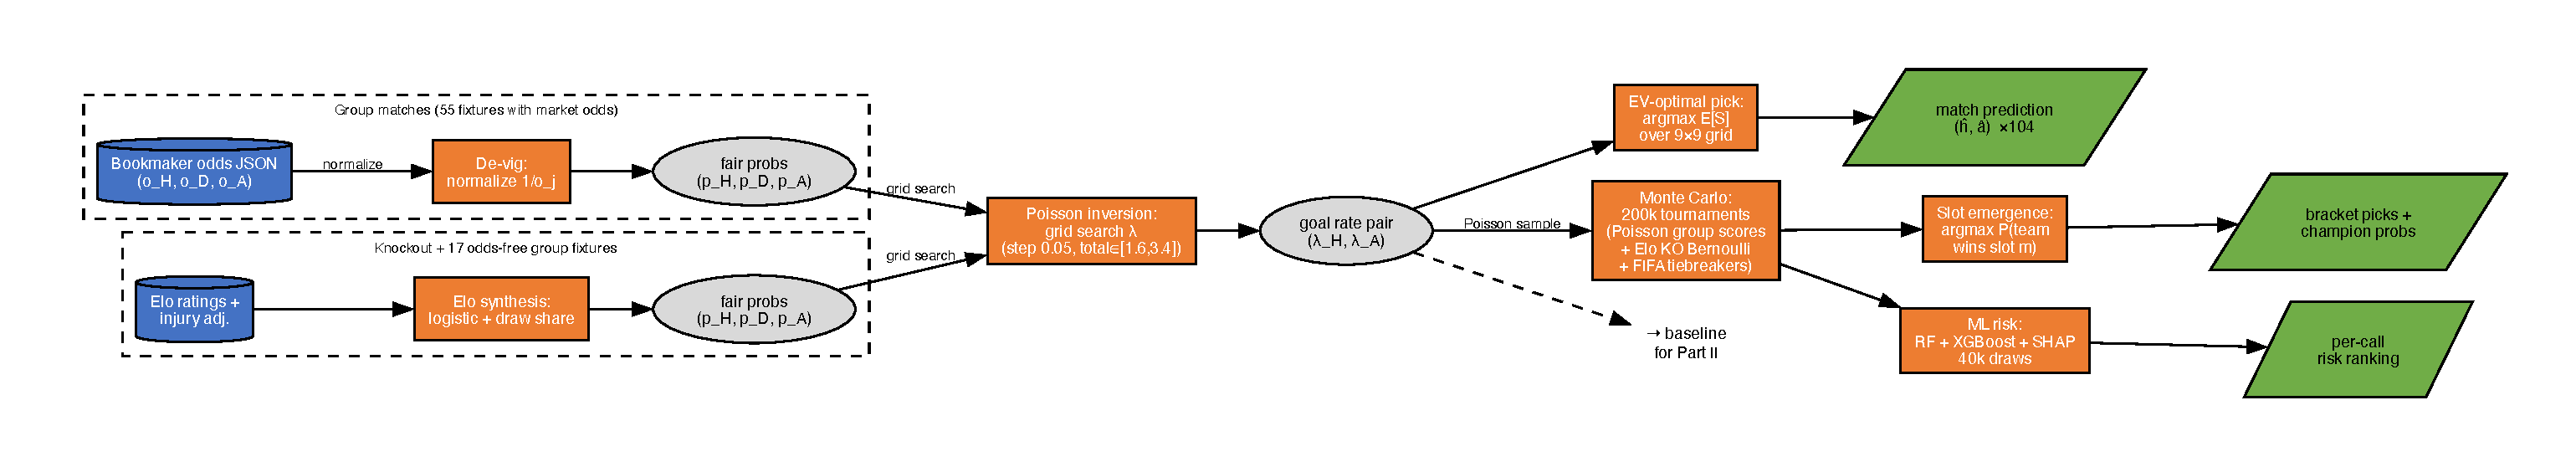
\includegraphics[width=\textwidth]{figs/fig_pipeline_part1.pdf}
\caption{Part~I locked forecast pipeline in detail. Two input lanes (market odds
for group matches; Elo synthesis for knockout matches and the 17 odds-free group
fixtures) merge at the fitted goal-rate pair $(\lambda_H, \lambda_A)$, which
feeds both the EV-optimal match prediction and the 200k-tournament Monte Carlo.}
\label{fig:part1}
\end{figure}

\part{The Live Prophet}

\section{Measurement: from match events to \texorpdfstring{$\lambda_{\mathrm{obs}}$}{lambda-obs}}
\label{sec:lambdaobs}
Real xG is not freely available for World Cups. The free signal that survives
is the box score: shots on target and other shots. Define the observed
performance rate of a team as
\begin{equation}
\hat\lambda_{\mathrm{obs}} = \max\!\bigl(0,\;
\beta_1\cdot\mathrm{SoT}+\beta_2\cdot\mathrm{otherShots}\bigr),
\qquad \beta_1=0.3256,\quad\beta_2=0,
\label{eq:proxy}
\end{equation}
where $\mathrm{otherShots}=\text{off-target}+\text{blocked}$.
The calibrated $\beta_2$ is exactly zero: each shot on target is worth about
a third of an expected goal; off-target and blocked shots carry no incremental
information once shots on target are counted.

\paragraph{Calibration.} The coefficients are a one-time least-squares fit of
realised goals on shot counts over the 2018 and 2022 World Cups
($n=236$ team-matches of free ESPN box-score data):
\begin{equation}
(\beta_1,\beta_2) = \underset{\beta\ge0}{\arg\min}
\sum_{i=1}^{236}\bigl(\mathrm{goals}_i
-\beta_1\,\mathrm{SoT}_i-\beta_2\,\mathrm{otherShots}_i\bigr)^2,
\label{eq:calibrate}
\end{equation}
OLS through the origin, clipped to non-negative coefficients.

\anchor{scripts/performance.py:proxy\_xg; coefficients in
data/proxy\_coef.json --- \texttt{sot: 0.32557, other: 0.0}.}

\paragraph{Fallback.} If a real xG number is available for a match, it takes
precedence, with the source recorded per match so the two never mix silently.

\anchor{scripts/performance.py:compute\_lambda\_obs ---
\texttt{source: 'real' | 'proxy'}.}

\section{The expectation model: \texorpdfstring{$\lambda_{\mathrm{exp}}$}{lambda-exp} from ratings}
\label{sec:lambdaexp}
Given two teams' current ratings, the expected performance rates are produced
by the same chain Part~I uses for odds-free matchups --- one composition of
three maps applied to the rating difference $d=R_{\mathrm{home}}-R_{\mathrm{away}}$:
\begin{equation}
d
\xrightarrow[\text{Elo logistic + draw}]{\text{(i)}}
(p_H,p_D,p_A)
\xrightarrow[\texttt{fit\_rates}]{\text{(ii)}}
(\lambda_{\mathrm{exp}}^{\mathrm{home}},\lambda_{\mathrm{exp}}^{\mathrm{away}}),
\label{eq:lambdaexp}
\end{equation}
where step~(i) is the synthesis of equations~\eqref{eq:elowin}--\eqref{eq:eloaway}
and step~(ii) is the lattice least-squares inversion of equation~\eqref{eq:fitrates}.
Nothing new is fitted here: the Prophet inherits Part~I's match model wholesale.

\paragraph{Numerics.} $\lambda_{\mathrm{exp}}$ depends only on $d$ rounded to
the nearest integer Elo point, and \texttt{\_lambda\_for\_diff} is memoised on
that integer. A half-point rating change moves the win expectancy by under
$10^{-3}$, far below the lattice resolution (0.05 goals) of the inversion it
feeds, so the cache is lossless in effect.

\anchor{scripts/learn.py:\_lambda\_for\_diff/lambda\_expected.}

\section{The learning update: net surprise and regularized drift}
\label{sec:drift}
\subsection*{Net surprise}
After a match, each team's performance is compared to expectation on both sides
of the ball and netted:
\begin{equation}
s_{\mathrm{home}} =
\underbrace{\bigl(\lambda_{\mathrm{obs}}^H-\lambda_{\mathrm{exp}}^H\bigr)}_{\text{attack surplus}}
-\underbrace{\bigl(\lambda_{\mathrm{obs}}^A-\lambda_{\mathrm{exp}}^A\bigr)}_{\text{defence leak}},
\qquad s_{\mathrm{away}}=-s_{\mathrm{home}}.
\label{eq:surprise}
\end{equation}
The construction is zero-sum by definition: one team's positive surprise is
exactly the other's negative, so learning redistributes strength rather than
inflating it.

\anchor{scripts/learn.py:net\_surprise and LearningTrack.apply\_match.}

\subsection*{The drift update}
Each team carries an accumulated drift $d_i$ (initialised to 0) on top of its
frozen baseline, $R_i^{\mathrm{learn}}=R_i+d_i$. One match updates it as
\begin{equation}
d_i \leftarrow \gamma\,d_i +
\operatorname{clip}(k\,s_i,\,-B,\,+B),
\qquad k=50,\quad\gamma=0.95,\quad B=75.
\label{eq:drift}
\end{equation}
The clip binds the per-match \emph{step} $ks_i$, not the accumulated drift.
Setting $k=0$ makes the step vanish and the drift stay at zero: the frozen
track is exactly the learning track at zero gain, which is what makes the A/B
comparison clean.

\anchor{scripts/learn.py:update\_drift ---
\texttt{step = max(-bound, min(bound, k*surprise)); return decay*drift + step};
defaults in \texttt{LearningTrack.\_\_init\_\_} (\texttt{k=50.0, decay=0.95, bound=75.0}).}

\section{Re-simulation and the two-track trajectory}
\label{sec:twotrack}
After $t$ games have been played, the forecast is the conditional distribution
\begin{equation}
p_t(\text{team}) = P\bigl(\text{team wins}\;\big|\;
\mathrm{results}_{1..t},\;\mathrm{ratings}_t\bigr),
\label{eq:cond}
\end{equation}
estimated by Monte Carlo with played games pinned and the future sampled.
The two tracks differ \emph{only} in $\mathrm{ratings}_t$: the frozen track
always passes the locked baseline $R_i$; the learning track passes
$R_i+d_{i,t}$ with the drift of \S\ref{sec:drift}.

\paragraph{The replay loop.} \texttt{run\_replay} steps an ordered game list.
For each finished game it (i) pins the result, (ii) applies the drift update
from the game's $\lambda_{\mathrm{obs}}$, and (iii) re-simulates the whole
tournament twice --- once per track --- recording a snapshot
$(p_t^{\mathrm{frozen}},p_t^{\mathrm{learn}})$. The trajectory is
\begin{equation}
\text{trajectory} =
\Bigl\{\bigl(p_t^{\mathrm{frozen}},p_t^{\mathrm{learn}}\bigr)\Bigr\}_{t=0}^{T},
\qquad\text{headline} = \text{the gap between the two paths.}
\label{eq:traj}
\end{equation}

\anchor{scripts/replay.py:run\_replay --- $N=4{,}000$ per snapshot, seed 2026.}

\section{Information accounting: KL divergence in bits}
\label{sec:kl}
Each snapshot records how far the new champion distribution moved from the
previous one, in bits:
\begin{equation}
D_{\mathrm{KL}}\bigl(p_t\,\big\|\,p_{t-1}\bigr)
= \sum_{i:\,p_t(i)>0}p_t(i)\,\log_2\frac{p_t(i)}{\max(p_{t-1}(i),\varepsilon)},
\qquad\varepsilon=10^{-12}.
\label{eq:kl}
\end{equation}
Base 2 makes the unit \textbf{bits}: one bit is the information in one fair
coin flip about the championship. This is the \emph{realised} counterpart of
\S\ref{sec:slot}'s pivotality: pivotality is the expected KL before kickoff;
\texttt{kl\_from\_prev} is what the match actually delivered.

\paragraph{Channel decomposition.}
\begin{itemize}
\item \textbf{Result channel}: the frozen track's own per-game divergence,
summed over a window --- what conditioning on scorelines alone teaches.
\item \textbf{Performance channel}:
$D_{\mathrm{KL}}(p_T^{\mathrm{learn}}\|p_T^{\mathrm{frozen}})$ --- what
reading the shot counts added beyond the scorelines.
\end{itemize}
Across the 48 group games of the 2022 replay the per-game result and
performance informations correlate at $-0.09$ --- essentially orthogonal. That
near-orthogonality is the empirical licence for the learning track's existence.

\anchor{scripts/snapshot.py:kl\_divergence; attached per snapshot as
\texttt{kl\_from\_prev} in scripts/replay.py:\_snapshot.}

\section{How we know it works: validation}
\label{sec:validation}
The learning claim was stress-tested against the two complete free-data
tournaments available, 2018 and 2022. The evaluation metric is
\textbf{finalist lift}: replay a tournament's group stage, then compare how
much champion-probability mass each track's end-of-groups forecast assigns to
the two teams that actually reached that final,
\begin{equation}
\mathrm{lift} =
\Bigl(\sum_{t\in\mathrm{finalists}}p_T^{\mathrm{learn}}(t)\Bigr)
-\Bigl(\sum_{t\in\mathrm{finalists}}p_T^{\mathrm{frozen}}(t)\Bigr)
\quad\text{percentage points.}
\label{eq:lift}
\end{equation}

\paragraph{(1) Leave-one-tournament-out cross-validation.}
Tune $k$ on one World Cup, test on the other. Train-2018 fixes $k=60$, tested
on 2022; train-2022 fixes $k=40$, tested on 2018. Learning helps out-of-sample
in both directions.

\anchor{scripts/heldout\_validation.py part~(1) --- $N=4{,}000$, seed~7.}

\paragraph{(2) Placebo control.}
Shuffle the $\lambda_{\mathrm{obs}}$ values across the tournament's games
(4 independent shuffles, seeds 0--3) and re-run at the locked $k=50$. The
real-xG lift collapses to negative territory under shuffling, confirming the
proxy carries real per-team information.

\anchor{scripts/heldout\_validation.py part~(2) --- \texttt{rng.shuffle(lams)},
$N=3{,}000$ per run.}

\paragraph{(3) Proxy stability.}
The $\beta_1$ coefficient refit on each tournament alone brackets the locked
value (0.326); the cross-tournament goal RMSE beats the naive baseline
(predict every team-match with the tournament mean goals) in both tournaments.

\anchor{scripts/heldout\_validation.py part~(3) --- per-tournament refit
$c=\sum s_ig_i/\sum s_i^2$ (OLS through the origin), RMSE comparisons.}

\paragraph{The $k$-sweep.}
Gain swept over $k\in\{0,20,40,60,80,120,160,220,300\}$ on full two-track
replays of both tournaments. The curve is single-peaked in both years ---
learning helps, then over-reacts. Optima: $k=40$ (2022), $k=60$ (2018);
locked default: midpoint $k=50$.

\anchor{scripts/sweep\_k.py ($N=3{,}000$, seed 2022),
scripts/run\_2018\_ksweep.py, figure paper/figs/fig\_ksweep\_2tourn.pdf.}

\paragraph{Limitations.}
The sample is $n=2$ tournaments; every number above carries that caveat. The
validation shows the learning signal is real and correctly signed out-of-sample
--- it does not pin the optimal gain to better than ``somewhere around 50,'' and
the study is framed as exploratory in the paper accordingly. The 2026 live run
is the genuine test.

\begin{figure}[H]
\centering
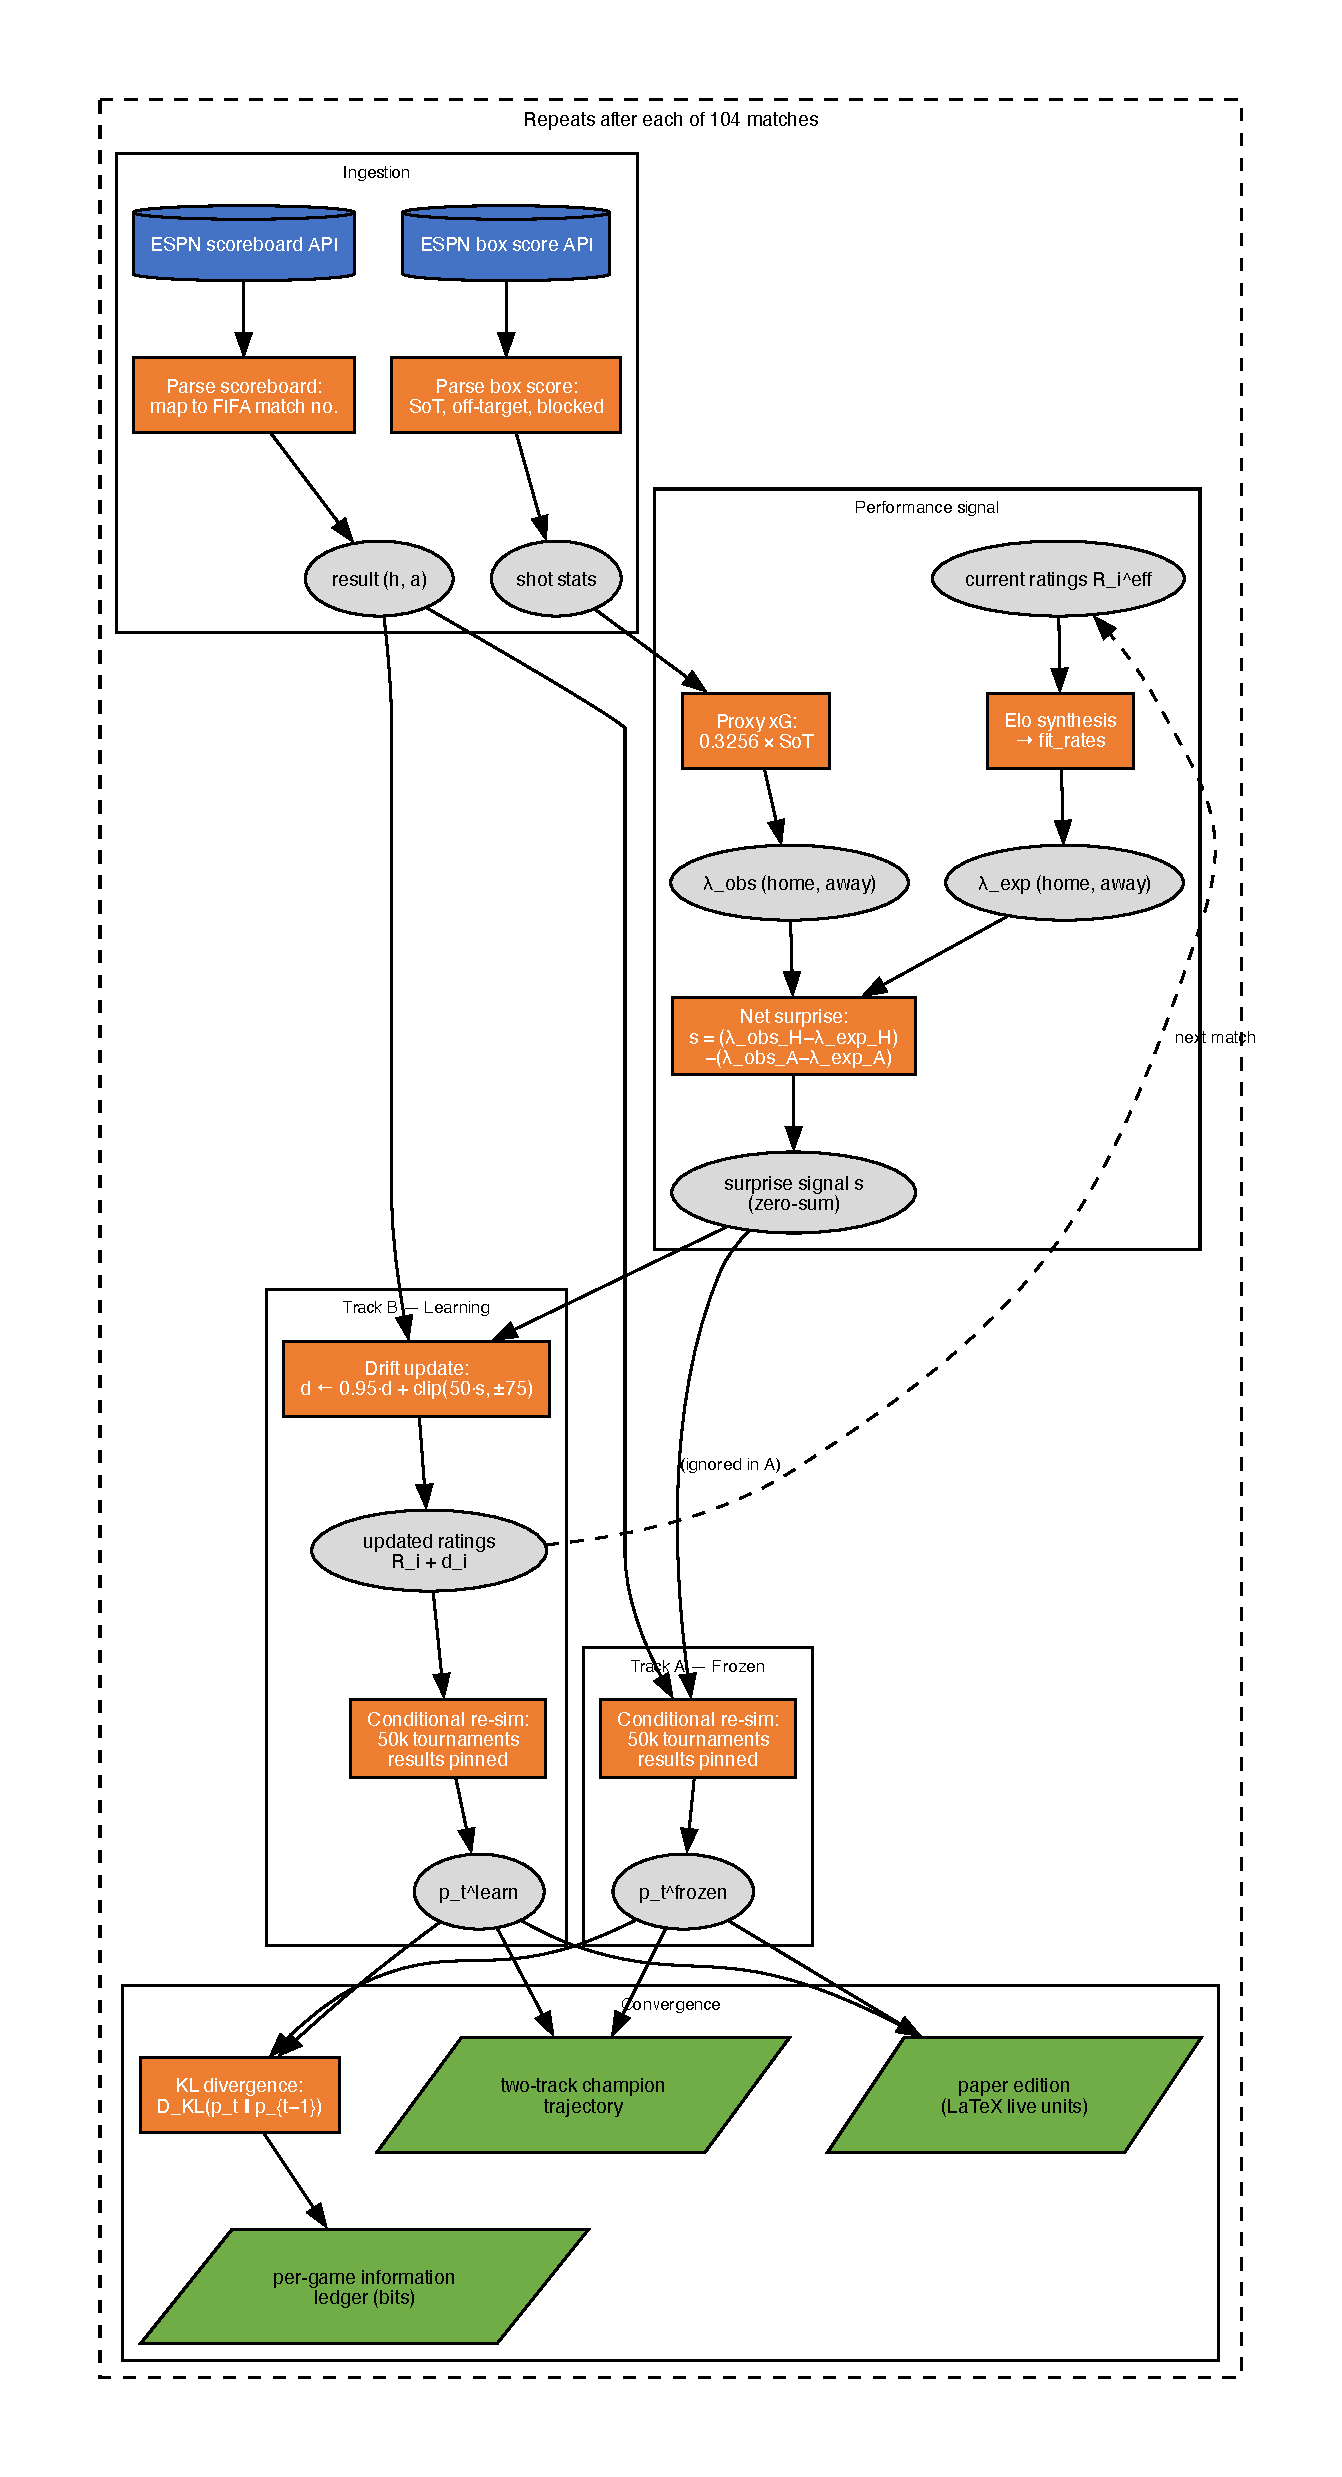
\includegraphics[width=\textwidth]{figs/fig_pipeline_part2.pdf}
\caption{Part~II live Prophet pipeline in detail. After each match, ESPN APIs
supply the result and shot statistics. Track~A (frozen) conditions on results
with fixed ratings; Track~B (learning) first updates per-team rating drift from
the observed/expected goal-rate gap, then conditions. The dashed feedback arrow
marks the cross-match accumulation of drift.}
\label{fig:part2}
\end{figure}

\end{document}
